% Created by tikzDevice version 0.12.3.1 on 2021-05-07 11:10:00
% !TEX encoding = UTF-8 Unicode
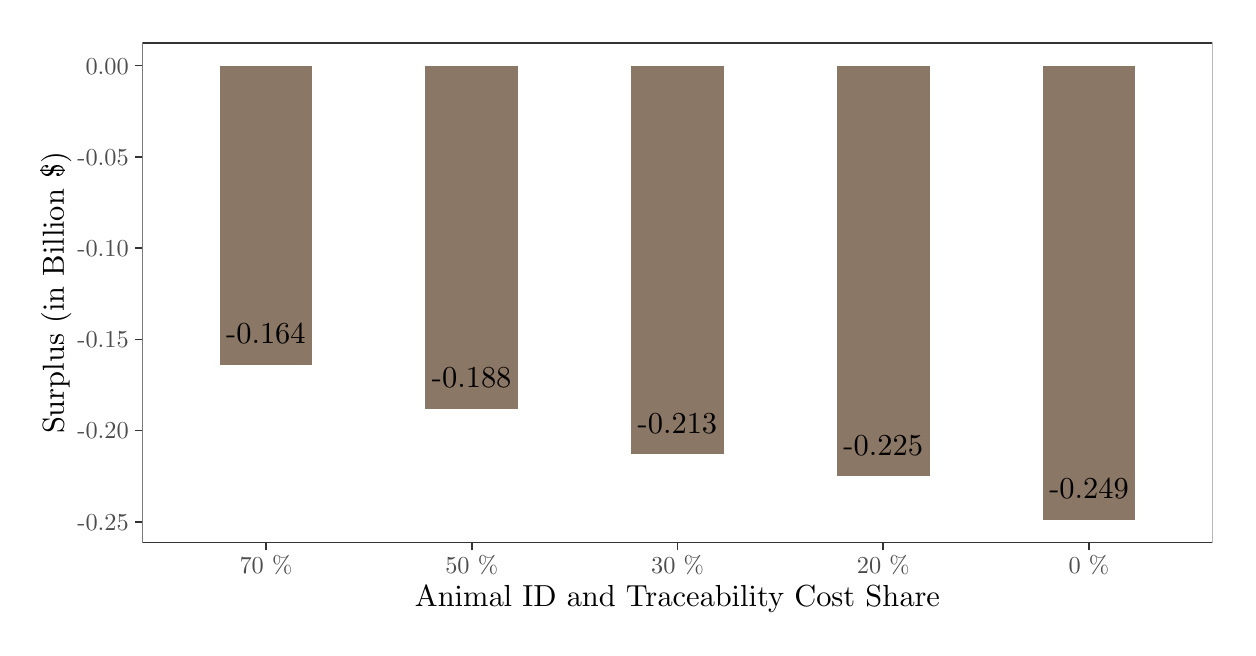
\begin{tikzpicture}[x=1pt,y=1pt]
\definecolor{fillColor}{RGB}{255,255,255}
\path[use as bounding box,fill=fillColor,fill opacity=0.00] (0,0) rectangle (433.62,216.81);
\begin{scope}
\path[clip] (  0.00,  0.00) rectangle (433.62,216.81);
\definecolor{drawColor}{RGB}{255,255,255}
\definecolor{fillColor}{RGB}{255,255,255}

\path[draw=drawColor,line width= 0.6pt,line join=round,line cap=round,fill=fillColor] (  0.00,  0.00) rectangle (433.62,216.81);
\end{scope}
\begin{scope}
\path[clip] ( 41.49, 30.69) rectangle (428.12,211.31);
\definecolor{fillColor}{RGB}{255,255,255}

\path[fill=fillColor] ( 41.49, 30.69) rectangle (428.12,211.31);
\definecolor{fillColor}{RGB}{139,119,101}

\path[fill=fillColor] (366.78, 38.90) rectangle (400.24,203.10);

\path[fill=fillColor] (292.43, 54.72) rectangle (325.89,203.10);

\path[fill=fillColor] (218.07, 62.64) rectangle (251.53,203.10);

\path[fill=fillColor] (143.72, 79.12) rectangle (177.18,203.10);

\path[fill=fillColor] ( 69.37, 94.95) rectangle (102.83,203.10);
\definecolor{drawColor}{RGB}{0,0,0}

\node[text=drawColor,anchor=base,inner sep=0pt, outer sep=0pt, scale=  1.10] at (383.51, 46.50) {-0.249};

\node[text=drawColor,anchor=base,inner sep=0pt, outer sep=0pt, scale=  1.10] at (309.16, 62.33) {-0.225};

\node[text=drawColor,anchor=base,inner sep=0pt, outer sep=0pt, scale=  1.10] at (234.80, 70.24) {-0.213};

\node[text=drawColor,anchor=base,inner sep=0pt, outer sep=0pt, scale=  1.10] at (160.45, 86.73) {-0.188};

\node[text=drawColor,anchor=base,inner sep=0pt, outer sep=0pt, scale=  1.10] at ( 86.10,102.55) {-0.164};
\definecolor{drawColor}{gray}{0.20}

\path[draw=drawColor,line width= 0.6pt,line join=round,line cap=round] ( 41.49, 30.69) rectangle (428.12,211.31);
\end{scope}
\begin{scope}
\path[clip] (  0.00,  0.00) rectangle (433.62,216.81);
\definecolor{drawColor}{gray}{0.30}

\node[text=drawColor,anchor=base east,inner sep=0pt, outer sep=0pt, scale=  0.88] at ( 36.54, 35.21) {-0.25};

\node[text=drawColor,anchor=base east,inner sep=0pt, outer sep=0pt, scale=  0.88] at ( 36.54, 68.18) {-0.20};

\node[text=drawColor,anchor=base east,inner sep=0pt, outer sep=0pt, scale=  0.88] at ( 36.54,101.15) {-0.15};

\node[text=drawColor,anchor=base east,inner sep=0pt, outer sep=0pt, scale=  0.88] at ( 36.54,134.12) {-0.10};

\node[text=drawColor,anchor=base east,inner sep=0pt, outer sep=0pt, scale=  0.88] at ( 36.54,167.10) {-0.05};

\node[text=drawColor,anchor=base east,inner sep=0pt, outer sep=0pt, scale=  0.88] at ( 36.54,200.07) {0.00};
\end{scope}
\begin{scope}
\path[clip] (  0.00,  0.00) rectangle (433.62,216.81);
\definecolor{drawColor}{gray}{0.20}

\path[draw=drawColor,line width= 0.6pt,line join=round] ( 38.74, 38.24) --
	( 41.49, 38.24);

\path[draw=drawColor,line width= 0.6pt,line join=round] ( 38.74, 71.21) --
	( 41.49, 71.21);

\path[draw=drawColor,line width= 0.6pt,line join=round] ( 38.74,104.18) --
	( 41.49,104.18);

\path[draw=drawColor,line width= 0.6pt,line join=round] ( 38.74,137.15) --
	( 41.49,137.15);

\path[draw=drawColor,line width= 0.6pt,line join=round] ( 38.74,170.13) --
	( 41.49,170.13);

\path[draw=drawColor,line width= 0.6pt,line join=round] ( 38.74,203.10) --
	( 41.49,203.10);
\end{scope}
\begin{scope}
\path[clip] (  0.00,  0.00) rectangle (433.62,216.81);
\definecolor{drawColor}{gray}{0.20}

\path[draw=drawColor,line width= 0.6pt,line join=round] ( 86.10, 27.94) --
	( 86.10, 30.69);

\path[draw=drawColor,line width= 0.6pt,line join=round] (160.45, 27.94) --
	(160.45, 30.69);

\path[draw=drawColor,line width= 0.6pt,line join=round] (234.80, 27.94) --
	(234.80, 30.69);

\path[draw=drawColor,line width= 0.6pt,line join=round] (309.16, 27.94) --
	(309.16, 30.69);

\path[draw=drawColor,line width= 0.6pt,line join=round] (383.51, 27.94) --
	(383.51, 30.69);
\end{scope}
\begin{scope}
\path[clip] (  0.00,  0.00) rectangle (433.62,216.81);
\definecolor{drawColor}{gray}{0.30}

\node[text=drawColor,anchor=base,inner sep=0pt, outer sep=0pt, scale=  0.88] at ( 86.10, 19.68) {70 \%};

\node[text=drawColor,anchor=base,inner sep=0pt, outer sep=0pt, scale=  0.88] at (160.45, 19.68) {50 \%};

\node[text=drawColor,anchor=base,inner sep=0pt, outer sep=0pt, scale=  0.88] at (234.80, 19.68) {30 \%};

\node[text=drawColor,anchor=base,inner sep=0pt, outer sep=0pt, scale=  0.88] at (309.16, 19.68) {20 \%};

\node[text=drawColor,anchor=base,inner sep=0pt, outer sep=0pt, scale=  0.88] at (383.51, 19.68) {0 \%};
\end{scope}
\begin{scope}
\path[clip] (  0.00,  0.00) rectangle (433.62,216.81);
\definecolor{drawColor}{RGB}{0,0,0}

\node[text=drawColor,anchor=base,inner sep=0pt, outer sep=0pt, scale=  1.10] at (234.80,  7.64) {Animal ID and Traceability Cost Share};
\end{scope}
\begin{scope}
\path[clip] (  0.00,  0.00) rectangle (433.62,216.81);
\definecolor{drawColor}{RGB}{0,0,0}

\node[text=drawColor,rotate= 90.00,anchor=base,inner sep=0pt, outer sep=0pt, scale=  1.10] at ( 13.08,121.00) {Surplus (in Billion \$)};
\end{scope}
\end{tikzpicture}
